\documentclass[12pt,]{article}
\usepackage{lmodern}
\usepackage{amssymb,amsmath}
\usepackage{ifxetex,ifluatex}
\usepackage{fixltx2e} % provides \textsubscript
\ifnum 0\ifxetex 1\fi\ifluatex 1\fi=0 % if pdftex
  \usepackage[T1]{fontenc}
  \usepackage[utf8]{inputenc}
\else % if luatex or xelatex
  \ifxetex
    \usepackage{mathspec}
  \else
    \usepackage{fontspec}
  \fi
  \defaultfontfeatures{Ligatures=TeX,Scale=MatchLowercase}
    \setmonofont[Mapping=tex-ansi,Scale=0.7]{Source Code Pro}
\fi
% use upquote if available, for straight quotes in verbatim environments
\IfFileExists{upquote.sty}{\usepackage{upquote}}{}
% use microtype if available
\IfFileExists{microtype.sty}{%
\usepackage{microtype}
\UseMicrotypeSet[protrusion]{basicmath} % disable protrusion for tt fonts
}{}
\usepackage[margin=1in]{geometry}
\usepackage{hyperref}
\PassOptionsToPackage{usenames,dvipsnames}{color} % color is loaded by hyperref
\hypersetup{unicode=true,
            pdftitle={Biostatistics using R},
            pdfauthor={Dewey Brooke},
            colorlinks=true,
            linkcolor=Maroon,
            citecolor=Blue,
            urlcolor=Blue,
            breaklinks=true}
\urlstyle{same}  % don't use monospace font for urls
\usepackage{natbib}
\bibliographystyle{apalike}
\usepackage{color}
\usepackage{fancyvrb}
\newcommand{\VerbBar}{|}
\newcommand{\VERB}{\Verb[commandchars=\\\{\}]}
\DefineVerbatimEnvironment{Highlighting}{Verbatim}{commandchars=\\\{\}}
% Add ',fontsize=\small' for more characters per line
\usepackage{framed}
\definecolor{shadecolor}{RGB}{248,248,248}
\newenvironment{Shaded}{\begin{snugshade}}{\end{snugshade}}
\newcommand{\KeywordTok}[1]{\textcolor[rgb]{0.13,0.29,0.53}{\textbf{#1}}}
\newcommand{\DataTypeTok}[1]{\textcolor[rgb]{0.13,0.29,0.53}{#1}}
\newcommand{\DecValTok}[1]{\textcolor[rgb]{0.00,0.00,0.81}{#1}}
\newcommand{\BaseNTok}[1]{\textcolor[rgb]{0.00,0.00,0.81}{#1}}
\newcommand{\FloatTok}[1]{\textcolor[rgb]{0.00,0.00,0.81}{#1}}
\newcommand{\ConstantTok}[1]{\textcolor[rgb]{0.00,0.00,0.00}{#1}}
\newcommand{\CharTok}[1]{\textcolor[rgb]{0.31,0.60,0.02}{#1}}
\newcommand{\SpecialCharTok}[1]{\textcolor[rgb]{0.00,0.00,0.00}{#1}}
\newcommand{\StringTok}[1]{\textcolor[rgb]{0.31,0.60,0.02}{#1}}
\newcommand{\VerbatimStringTok}[1]{\textcolor[rgb]{0.31,0.60,0.02}{#1}}
\newcommand{\SpecialStringTok}[1]{\textcolor[rgb]{0.31,0.60,0.02}{#1}}
\newcommand{\ImportTok}[1]{#1}
\newcommand{\CommentTok}[1]{\textcolor[rgb]{0.56,0.35,0.01}{\textit{#1}}}
\newcommand{\DocumentationTok}[1]{\textcolor[rgb]{0.56,0.35,0.01}{\textbf{\textit{#1}}}}
\newcommand{\AnnotationTok}[1]{\textcolor[rgb]{0.56,0.35,0.01}{\textbf{\textit{#1}}}}
\newcommand{\CommentVarTok}[1]{\textcolor[rgb]{0.56,0.35,0.01}{\textbf{\textit{#1}}}}
\newcommand{\OtherTok}[1]{\textcolor[rgb]{0.56,0.35,0.01}{#1}}
\newcommand{\FunctionTok}[1]{\textcolor[rgb]{0.00,0.00,0.00}{#1}}
\newcommand{\VariableTok}[1]{\textcolor[rgb]{0.00,0.00,0.00}{#1}}
\newcommand{\ControlFlowTok}[1]{\textcolor[rgb]{0.13,0.29,0.53}{\textbf{#1}}}
\newcommand{\OperatorTok}[1]{\textcolor[rgb]{0.81,0.36,0.00}{\textbf{#1}}}
\newcommand{\BuiltInTok}[1]{#1}
\newcommand{\ExtensionTok}[1]{#1}
\newcommand{\PreprocessorTok}[1]{\textcolor[rgb]{0.56,0.35,0.01}{\textit{#1}}}
\newcommand{\AttributeTok}[1]{\textcolor[rgb]{0.77,0.63,0.00}{#1}}
\newcommand{\RegionMarkerTok}[1]{#1}
\newcommand{\InformationTok}[1]{\textcolor[rgb]{0.56,0.35,0.01}{\textbf{\textit{#1}}}}
\newcommand{\WarningTok}[1]{\textcolor[rgb]{0.56,0.35,0.01}{\textbf{\textit{#1}}}}
\newcommand{\AlertTok}[1]{\textcolor[rgb]{0.94,0.16,0.16}{#1}}
\newcommand{\ErrorTok}[1]{\textcolor[rgb]{0.64,0.00,0.00}{\textbf{#1}}}
\newcommand{\NormalTok}[1]{#1}
\usepackage{longtable,booktabs}
\usepackage{graphicx,grffile}
\makeatletter
\def\maxwidth{\ifdim\Gin@nat@width>\linewidth\linewidth\else\Gin@nat@width\fi}
\def\maxheight{\ifdim\Gin@nat@height>\textheight\textheight\else\Gin@nat@height\fi}
\makeatother
% Scale images if necessary, so that they will not overflow the page
% margins by default, and it is still possible to overwrite the defaults
% using explicit options in \includegraphics[width, height, ...]{}
\setkeys{Gin}{width=\maxwidth,height=\maxheight,keepaspectratio}
\IfFileExists{parskip.sty}{%
\usepackage{parskip}
}{% else
\setlength{\parindent}{0pt}
\setlength{\parskip}{6pt plus 2pt minus 1pt}
}
\setlength{\emergencystretch}{3em}  % prevent overfull lines
\providecommand{\tightlist}{%
  \setlength{\itemsep}{0pt}\setlength{\parskip}{0pt}}
\setcounter{secnumdepth}{5}
% Redefines (sub)paragraphs to behave more like sections
\ifx\paragraph\undefined\else
\let\oldparagraph\paragraph
\renewcommand{\paragraph}[1]{\oldparagraph{#1}\mbox{}}
\fi
\ifx\subparagraph\undefined\else
\let\oldsubparagraph\subparagraph
\renewcommand{\subparagraph}[1]{\oldsubparagraph{#1}\mbox{}}
\fi

%%% Use protect on footnotes to avoid problems with footnotes in titles
\let\rmarkdownfootnote\footnote%
\def\footnote{\protect\rmarkdownfootnote}

%%% Change title format to be more compact
\usepackage{titling}

% Create subtitle command for use in maketitle
\newcommand{\subtitle}[1]{
  \posttitle{
    \begin{center}\large#1\end{center}
    }
}

\setlength{\droptitle}{-2em}
  \title{Biostatistics using R}
  \pretitle{\vspace{\droptitle}\centering\huge}
  \posttitle{\par}
  \author{Dewey Brooke}
  \preauthor{\centering\large\emph}
  \postauthor{\par}
  \predate{\centering\large\emph}
  \postdate{\par}
  \date{2018-06-29}

\usepackage{booktabs}

\usepackage{amsthm}
\newtheorem{theorem}{Theorem}[section]
\newtheorem{lemma}{Lemma}[section]
\theoremstyle{definition}
\newtheorem{definition}{Definition}[section]
\newtheorem{corollary}{Corollary}[section]
\newtheorem{proposition}{Proposition}[section]
\theoremstyle{definition}
\newtheorem{example}{Example}[section]
\theoremstyle{definition}
\newtheorem{exercise}{Exercise}[section]
\theoremstyle{remark}
\newtheorem*{remark}{Remark}
\newtheorem*{solution}{Solution}
\begin{document}
\maketitle

{
\hypersetup{linkcolor=black}
\setcounter{tocdepth}{2}
\tableofcontents
}
\listoftables
\listoffigures
\section*{Preface}\label{preface}
\addcontentsline{toc}{section}{Preface}

This is a \emph{sample} book written in \textbf{Markdown}. You can use
anything that Pandoc's Markdown supports, e.g., a math equation
\(a^2 + b^2 = c^2\).

The \textbf{bookdown} package can be installed from CRAN or Github:

\begin{Shaded}
\begin{Highlighting}[]
\KeywordTok{install.packages}\NormalTok{(}\StringTok{"bookdown"}\NormalTok{)}
\CommentTok{# or the development version}
\CommentTok{# devtools::install_github("rstudio/bookdown")}
\end{Highlighting}
\end{Shaded}

Remember each Rmd file contains one and only one chapter, and a chapter
is defined by the first-level heading \texttt{\#}.

To compile this example to PDF, you need XeLaTeX. You are recommended to
install TinyTeX (which includes XeLaTeX):
\url{https://yihui.name/tinytex/}.

\section{Introduction}\label{intro}

You can label chapter and section titles using \texttt{\{\#label\}}
after them, e.g., we can reference Chapter \ref{intro}. If you do not
manually label them, there will be automatic labels anyway, e.g.,
Chapter \ref{methods}.

Figures and tables with captions will be placed in \texttt{figure} and
\texttt{table} environments, respectively.

\begin{Shaded}
\begin{Highlighting}[]
\KeywordTok{par}\NormalTok{(}\DataTypeTok{mar =} \KeywordTok{c}\NormalTok{(}\DecValTok{4}\NormalTok{, }\DecValTok{4}\NormalTok{, .}\DecValTok{1}\NormalTok{, .}\DecValTok{1}\NormalTok{))}
\KeywordTok{plot}\NormalTok{(pressure, }\DataTypeTok{type =} \StringTok{'b'}\NormalTok{, }\DataTypeTok{pch =} \DecValTok{19}\NormalTok{)}
\end{Highlighting}
\end{Shaded}

\begin{figure}

{\centering 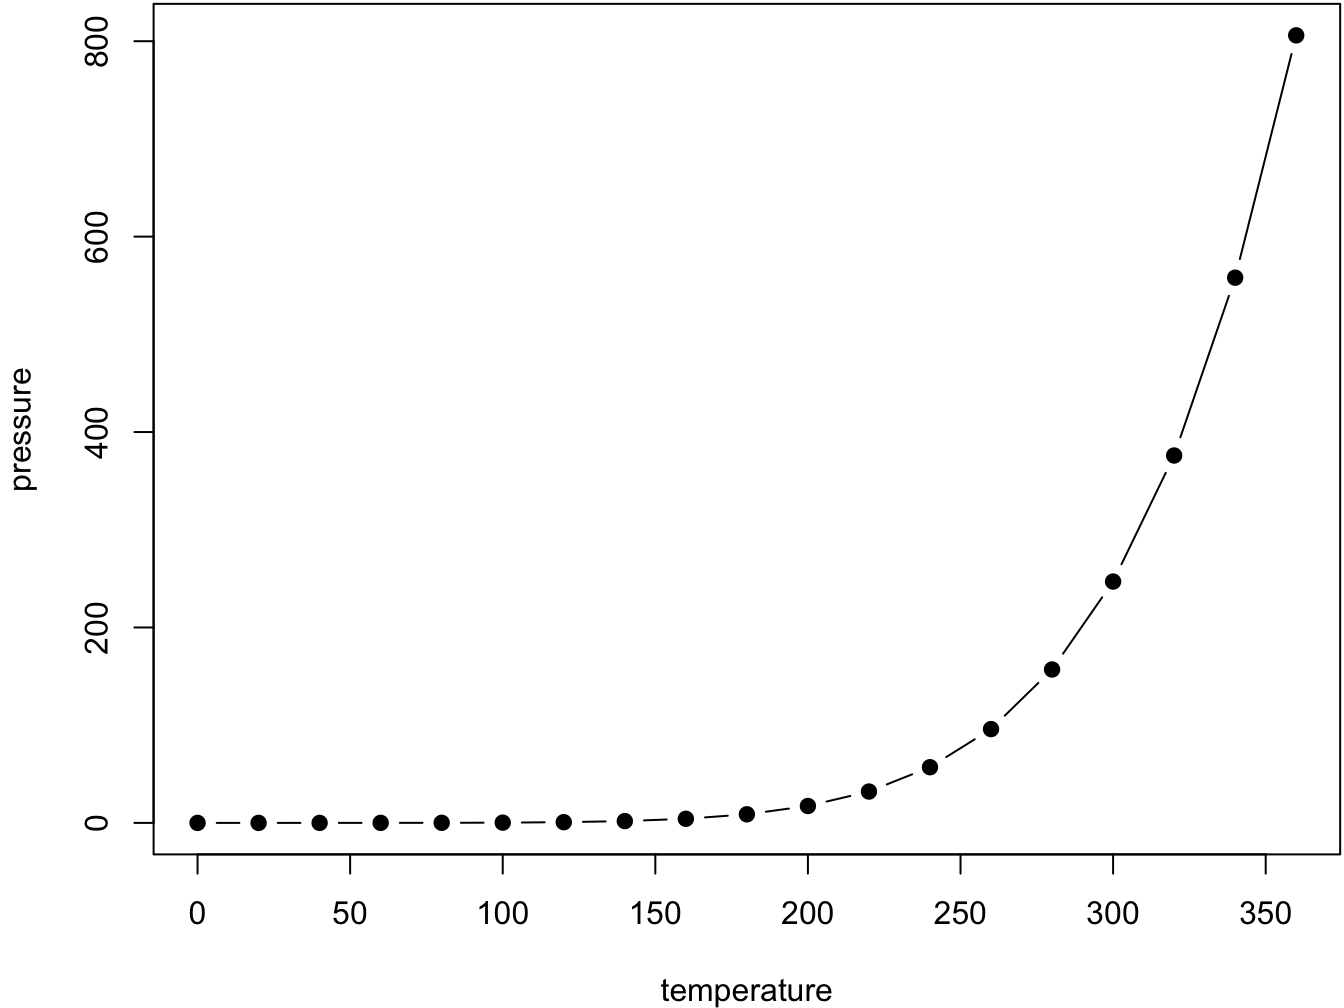
\includegraphics[width=0.8\linewidth]{bst4r_files/figure-latex/nice-fig-1} 

}

\caption{Here is a nice figure!}\label{fig:nice-fig}
\end{figure}

Reference a figure by its code chunk label with the \texttt{fig:}
prefix, e.g., see Figure \ref{fig:nice-fig}. Similarly, you can
reference tables generated from \texttt{knitr::kable()}, e.g., see Table
\ref{tab:nice-tab}.

\begin{Shaded}
\begin{Highlighting}[]
\NormalTok{knitr}\OperatorTok{::}\KeywordTok{kable}\NormalTok{(}
  \KeywordTok{head}\NormalTok{(iris, }\DecValTok{20}\NormalTok{), }\DataTypeTok{caption =} \StringTok{'Here is a nice table!'}\NormalTok{,}
  \DataTypeTok{booktabs =} \OtherTok{TRUE}
\NormalTok{)}
\end{Highlighting}
\end{Shaded}

\begin{table}

\caption{\label{tab:nice-tab}Here is a nice table!}
\centering
\begin{tabular}[t]{rrrrl}
\toprule
Sepal.Length & Sepal.Width & Petal.Length & Petal.Width & Species\\
\midrule
5.1 & 3.5 & 1.4 & 0.2 & setosa\\
4.9 & 3.0 & 1.4 & 0.2 & setosa\\
4.7 & 3.2 & 1.3 & 0.2 & setosa\\
4.6 & 3.1 & 1.5 & 0.2 & setosa\\
5.0 & 3.6 & 1.4 & 0.2 & setosa\\
\addlinespace
5.4 & 3.9 & 1.7 & 0.4 & setosa\\
4.6 & 3.4 & 1.4 & 0.3 & setosa\\
5.0 & 3.4 & 1.5 & 0.2 & setosa\\
4.4 & 2.9 & 1.4 & 0.2 & setosa\\
4.9 & 3.1 & 1.5 & 0.1 & setosa\\
\addlinespace
5.4 & 3.7 & 1.5 & 0.2 & setosa\\
4.8 & 3.4 & 1.6 & 0.2 & setosa\\
4.8 & 3.0 & 1.4 & 0.1 & setosa\\
4.3 & 3.0 & 1.1 & 0.1 & setosa\\
5.8 & 4.0 & 1.2 & 0.2 & setosa\\
\addlinespace
5.7 & 4.4 & 1.5 & 0.4 & setosa\\
5.4 & 3.9 & 1.3 & 0.4 & setosa\\
5.1 & 3.5 & 1.4 & 0.3 & setosa\\
5.7 & 3.8 & 1.7 & 0.3 & setosa\\
5.1 & 3.8 & 1.5 & 0.3 & setosa\\
\bottomrule
\end{tabular}
\end{table}

You can write citations, too. For example, we are using the
\textbf{bookdown} package \citep{R-bookdown} in this sample book, which
was built on top of R Markdown and \textbf{knitr} \citep{xie2015}.

\section*{Reading Data Files into R}\label{reading-data-files-into-r}
\addcontentsline{toc}{section}{Reading Data Files into R}

The first step in every analysis requires data to be read into the
environment, and learning how to do this is the first hurdle a person
needs to overcome to begin learning to use R.

Data can exist in many different formats, either as the generic
universal types (e.g.~csv, tsv, .json, etc) or software specific types
(e.g. \texttt{.xlsx}, `` )

In this chapter, we will first discuss how to read data using functions
in Base-R (when possible), and then we will discuss alternative
packages, such as the multitude of packages in the
\href{https://www.tidyverse.org}{Tidyverse}, and highlight their
advantages over Base-R functions.

\subsection{Generic Formats}\label{generic-formats}

\subsubsection{CSV- Comma Separated
Values}\label{csv--comma-separated-values}

The fields are separated by a comma \texttt{,} and are typically used
for loading into spreadsheets.

For example:

\begin{Shaded}
\begin{Highlighting}[]
\NormalTok{csv_example_path <-}\StringTok{ "data/ASCII-comma/FEV.DAT.txt"}

\KeywordTok{readLines}\NormalTok{(csv_example_path)[}\DecValTok{1}\OperatorTok{:}\DecValTok{8}\NormalTok{]  }\CommentTok{# reads each line of the file}
\end{Highlighting}
\end{Shaded}

\begin{verbatim}
[1] "'Id','Age','FEV','Hgt','Sex','Smoke'"
[2] "301,9,1.708,57,0,0"                  
[3] "451,8,1.724,67.5,0,0"                
[4] "501,7,1.72,54.5,0,0"                 
[5] "642,9,1.558,53,1,0"                  
[6] "901,9,1.895,57,1,0"                  
[7] "1701,8,2.336,61,0,0"                 
[8] "1752,6,1.919,58,0,0"                 
\end{verbatim}

\begin{Shaded}
\begin{Highlighting}[]
\CommentTok{# Note: readLines(csv_example_path) is the same as}
\CommentTok{# readLines("data/ASCII-comma/FEV.DAT.txt")}
\end{Highlighting}
\end{Shaded}

In Base-R, CSV data can be read using the \texttt{read.csv()} function.
The \texttt{read.csv2()} function is used in countires that use a comma
as a decimal point and a semicolon as a field separator.

\begin{Shaded}
\begin{Highlighting}[]
\NormalTok{csv_example <-}\StringTok{ }\KeywordTok{read.csv}\NormalTok{(csv_example_path)}

\KeywordTok{head}\NormalTok{(csv_example)}
\end{Highlighting}
\end{Shaded}

\begin{verbatim}
  X.Id. X.Age. X.FEV. X.Hgt. X.Sex. X.Smoke.
1   301      9  1.708   57.0      0        0
2   451      8  1.724   67.5      0        0
3   501      7  1.720   54.5      0        0
4   642      9  1.558   53.0      1        0
5   901      9  1.895   57.0      1        0
6  1701      8  2.336   61.0      0        0
\end{verbatim}

\subsubsection{TSV- Tab Separeted
Values}\label{tsv--tab-separeted-values}

The fields are separated by a tabulation or \t and are saved as
\texttt{.txt} files. However, not all \texttt{.txt} files contain tab
separated values.

For example:

\begin{Shaded}
\begin{Highlighting}[]
\NormalTok{tsv_example_path <-}\StringTok{ "data/ASCII-tab/FEV.DAT.txt"}

\KeywordTok{readLines}\NormalTok{(tsv_example_path)[}\DecValTok{1}\OperatorTok{:}\DecValTok{8}\NormalTok{]}
\end{Highlighting}
\end{Shaded}

\begin{verbatim}
[1] "'Id'\t'Age'\t'FEV'\t'Hgt'\t'Sex'\t'Smoke'"
[2] "301\t9\t1.708\t57\t0\t0"                  
[3] "451\t8\t1.724\t67.5\t0\t0"                
[4] "501\t7\t1.72\t54.5\t0\t0"                 
[5] "642\t9\t1.558\t53\t1\t0"                  
[6] "901\t9\t1.895\t57\t1\t0"                  
[7] "1701\t8\t2.336\t61\t0\t0"                 
[8] "1752\t6\t1.919\t58\t0\t0"                 
\end{verbatim}

\begin{Shaded}
\begin{Highlighting}[]
\NormalTok{tsv_example <-}\StringTok{ }\KeywordTok{read.delim}\NormalTok{(}\StringTok{"data/ASCII-tab/FEV.DAT.txt"}\NormalTok{)}
\KeywordTok{head}\NormalTok{(tsv_example)}
\end{Highlighting}
\end{Shaded}

\begin{verbatim}
  X.Id. X.Age. X.FEV. X.Hgt. X.Sex. X.Smoke.
1   301      9  1.708   57.0      0        0
2   451      8  1.724   67.5      0        0
3   501      7  1.720   54.5      0        0
4   642      9  1.558   53.0      1        0
5   901      9  1.895   57.0      1        0
6  1701      8  2.336   61.0      0        0
\end{verbatim}

\subsection{Excel}\label{excel}

\begin{Shaded}
\begin{Highlighting}[]
\KeywordTok{library}\NormalTok{(readxl)}
\end{Highlighting}
\end{Shaded}

\subsection{Software Specific Formats}\label{software-specific-formats}

R is increasingly recognized as the gold standard for statistical
computations, yet some of your future collaboraters will exclusively use
Commercial Software (SAS, SPSS, Matlab, and Stata) for their statistical
computations. Although these individuals are limited by the types of
files they can read or write, the \texttt{haven} R-package can both read
and write any of these file formats.

\begin{Shaded}
\begin{Highlighting}[]
\KeywordTok{library}\NormalTok{(haven)}
\end{Highlighting}
\end{Shaded}

\subsubsection{\texorpdfstring{SAS(\texttt{.sas7bdat}),
SPSS(\texttt{.sav},\texttt{.por}, \texttt{.xpt}), Stata
(\texttt{.dta})}{SAS(.sas7bdat), SPSS(.sav,.por, .xpt), Stata (.dta)}}\label{sas.sas7bdat-spss.sav.por-.xpt-stata-.dta}

\begin{Shaded}
\begin{Highlighting}[]
\NormalTok{sas <-}\StringTok{ }\KeywordTok{read_sas}\NormalTok{(}\StringTok{"data/SAS/FEV.sas7bdat"}\NormalTok{)}

\KeywordTok{head}\NormalTok{(sas)}
\end{Highlighting}
\end{Shaded}

\begin{verbatim}
# A tibble: 6 x 6
     ID   AGE   FEV   HGT   SEX SMOKE
  <dbl> <dbl> <dbl> <dbl> <dbl> <dbl>
1   301     9  1.71  57       0     0
2   451     8  1.72  67.5     0     0
3   501     7  1.72  54.5     0     0
4   642     9  1.56  53       1     0
5   901     9  1.90  57       1     0
6  1701     8  2.34  61       0     0
\end{verbatim}

\begin{Shaded}
\begin{Highlighting}[]
\NormalTok{spss <-}\StringTok{ }\KeywordTok{read_spss}\NormalTok{(}\StringTok{"data/SPSS/FEV.DAT.sav"}\NormalTok{)}
\KeywordTok{head}\NormalTok{(spss)}
\end{Highlighting}
\end{Shaded}

\begin{verbatim}
# A tibble: 6 x 6
     Id   Age   FEV   Hgt   Sex Smoke
  <dbl> <dbl> <dbl> <dbl> <dbl> <dbl>
1   301     9  1.71  57       0     0
2   451     8  1.72  67.5     0     0
3   501     7  1.72  54.5     0     0
4   642     9  1.56  53       1     0
5   901     9  1.90  57       1     0
6  1701     8  2.34  61       0     0
\end{verbatim}

\begin{Shaded}
\begin{Highlighting}[]
\NormalTok{stata <-}\StringTok{ }\KeywordTok{read_stata}\NormalTok{(}\StringTok{"data/Stata/FEV.DAT.dta"}\NormalTok{)}
\KeywordTok{head}\NormalTok{(stata)}
\end{Highlighting}
\end{Shaded}

\begin{verbatim}
# A tibble: 6 x 6
     Id   Age   fev   Hgt   Sex Smoke
  <dbl> <dbl> <dbl> <dbl> <dbl> <dbl>
1   301     9  1.71  57       0     0
2   451     8  1.72  67.5     0     0
3   501     7  1.72  54.5     0     0
4   642     9  1.56  53       1     0
5   901     9  1.90  57       1     0
6  1701     8  2.34  61       0     0
\end{verbatim}

The \texttt{foreign} package included in Base-R can also be used to
Reading and writing data stored by some versions of `Epi Info',
`Minitab', `S', `SAS', `SPSS', `Stata', `Systat', `Weka',and for reading
and writing some `dBase' files.

\paragraph{RDS}\label{rds}

\begin{Shaded}
\begin{Highlighting}[]
\NormalTok{rds_example <-}\StringTok{ }\KeywordTok{readRDS}\NormalTok{(}\StringTok{"data/RDS/BETACAR.DAT.rds"}\NormalTok{)}
\KeywordTok{head}\NormalTok{(rds_example)}
\end{Highlighting}
\end{Shaded}

\begin{verbatim}
# A tibble: 6 x 8
  `'Prepar'` `'Id'` `'Base1lvl'` `'Base2lvl'`
       <int>  <int>        <int>        <int>
1          1     71          298          116
2          1     73          124          146
3          1     80          176          200
4          1     83          116          180
5          1     90          152          142
6          1     92          106          106
# ... with 4 more variables: `'Wk6lvl'` <int>,
#   `'Wk8lvl'` <int>, `'Wk10lvl'` <int>,
#   `'Wk12lvl'` <int>
\end{verbatim}

\paragraph{\texorpdfstring{\texttt{rdata}}{rdata}}\label{rdata}

The \texttt{.rdata} format is R's specific format. Instead of using a
\texttt{read.\{something\}} function, \texttt{.rdata} is read into the
environment using \texttt{load(filename.rdata)} and retains the original
name it had when it was last saved.

\begin{Shaded}
\begin{Highlighting}[]
\KeywordTok{load}\NormalTok{(}\StringTok{"data/R/BETACAR.DAT.rdata"}\NormalTok{)  }\CommentTok{#named betacar when it was last saved}
\KeywordTok{head}\NormalTok{(betacar)}
\end{Highlighting}
\end{Shaded}

\begin{verbatim}
  Prepar Id Base1lvl Base2lvl Wk6lvl Wk8lvl Wk10lvl
1      1 71      298      116    174    178     218
2      1 73      124      146    294    278     244
3      1 80      176      200    276    286     308
4      1 83      116      180    164    238     308
5      1 90      152      142    290    300     270
6      1 92      106      106    246    206     304
  Wk12lvl
1     190
2     262
3     334
4     226
5     268
6     356
\end{verbatim}

\section{Chapter 2: Descriptive
Statistics}\label{chapter-2-descriptive-statistics}

\subsection{Introduction}\label{introduction}

\begin{verbatim}
PhantomJS not found. You can install it with webshot::install_phantomjs(). If it is installed, please make sure the phantomjs executable can be found via the PATH variable.
\end{verbatim}

\hypertarget{htmlwidget-d155486f8bf8de5b1cac}{}

\subsection{Measures of Location using Base
R}\label{measures-of-location-using-base-r}

\begin{Shaded}
\begin{Highlighting}[]
\KeywordTok{head}\NormalTok{(ChickWeight)}
\end{Highlighting}
\end{Shaded}

\begin{verbatim}
  weight Time Chick Diet
1     42    0     1    1
2     51    2     1    1
3     59    4     1    1
4     64    6     1    1
5     76    8     1    1
6     93   10     1    1
\end{verbatim}

\subsubsection{The Arithmetic Mean}\label{the-arithmetic-mean}

The arithmetic mean is the sum of all the observations divided by the
number of observations. It is written in statistical terms as

\[\overline{x} = \frac{1}{n}\sum^n_{i=1}x_i\]

\begin{Shaded}
\begin{Highlighting}[]
\NormalTok{y=}\StringTok{ }\KeywordTok{rbeta}\NormalTok{(}\DecValTok{10000}\NormalTok{,}\DecValTok{1}\NormalTok{,}\DecValTok{12}\NormalTok{,}\DecValTok{6}\NormalTok{)}
\KeywordTok{hist}\NormalTok{(y, }\CommentTok{# histogram}
 \DataTypeTok{col =} \StringTok{"lightblue"}\NormalTok{, }\CommentTok{# column color}
 \DataTypeTok{border =} \StringTok{"black"}\NormalTok{, }
 \DataTypeTok{prob =} \OtherTok{TRUE}\NormalTok{, }\CommentTok{# show densities instead of frequencies}
 \DataTypeTok{xlab =} \StringTok{"x"}\NormalTok{,}
 \DataTypeTok{ylim =} \KeywordTok{c}\NormalTok{(}\DecValTok{0}\NormalTok{,}\FloatTok{3.5}\NormalTok{),}
 \DataTypeTok{main =} \StringTok{"Skewed Dataset"}
\NormalTok{ )}

\KeywordTok{lines}\NormalTok{(}\KeywordTok{density}\NormalTok{(y), }\DataTypeTok{col=}\StringTok{'black'}\NormalTok{, }\DataTypeTok{lwd=}\DecValTok{3}\NormalTok{)}
\KeywordTok{abline}\NormalTok{(}\DataTypeTok{v =} \KeywordTok{mean}\NormalTok{(y),}
 \DataTypeTok{col =} \StringTok{"royalblue"}\NormalTok{,}
 \DataTypeTok{lwd =} \DecValTok{2}\NormalTok{)}

\KeywordTok{abline}\NormalTok{(}\DataTypeTok{v =} \KeywordTok{median}\NormalTok{(y),}
 \DataTypeTok{col =} \StringTok{"red"}\NormalTok{,}
 \DataTypeTok{lwd =} \DecValTok{2}\NormalTok{)}

\KeywordTok{abline}\NormalTok{(}\DataTypeTok{v =} \KeywordTok{exp}\NormalTok{(}\KeywordTok{mean}\NormalTok{(}\KeywordTok{log}\NormalTok{(y))),}
 \DataTypeTok{col =} \StringTok{"green"}\NormalTok{,}
 \DataTypeTok{lwd =} \DecValTok{2}\NormalTok{)}



\KeywordTok{legend}\NormalTok{(}\DataTypeTok{x =} \StringTok{"topright"}\NormalTok{, }\CommentTok{# location of legend within plot area}
 \KeywordTok{c}\NormalTok{(}\StringTok{"Mean"}\NormalTok{, }\StringTok{"Median"}\NormalTok{, }\StringTok{"Geometric Mean"}\NormalTok{),}
 \DataTypeTok{col =} \KeywordTok{c}\NormalTok{( }\StringTok{"royalblue"}\NormalTok{, }\StringTok{"red"}\NormalTok{, }\StringTok{"green"}\NormalTok{),}
 \DataTypeTok{lwd =} \KeywordTok{c}\NormalTok{(}\DecValTok{2}\NormalTok{, }\DecValTok{2}\NormalTok{, }\DecValTok{2}\NormalTok{))}
\end{Highlighting}
\end{Shaded}

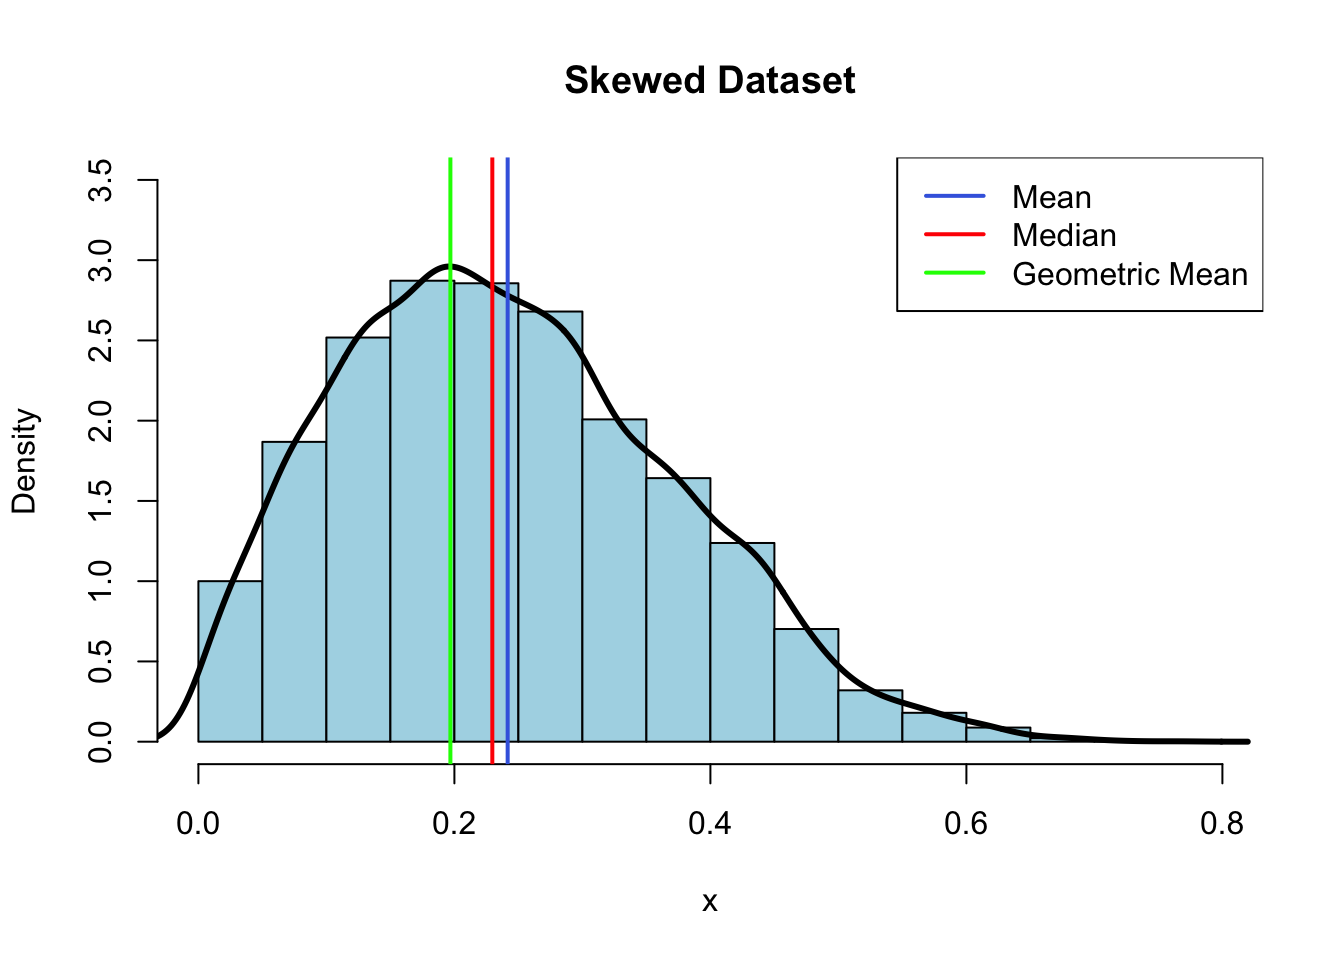
\includegraphics{bst4r_files/figure-latex/unnamed-chunk-13-1.pdf}

\begin{Shaded}
\begin{Highlighting}[]
\KeywordTok{mean}\NormalTok{(ChickWeight}\OperatorTok{$}\NormalTok{weight)}
\end{Highlighting}
\end{Shaded}

\begin{verbatim}
[1] 121.8
\end{verbatim}

\subsubsection{The Median}\label{the-median}

\begin{Shaded}
\begin{Highlighting}[]
\KeywordTok{median}\NormalTok{(ChickWeight}\OperatorTok{$}\NormalTok{weight)}
\end{Highlighting}
\end{Shaded}

\begin{verbatim}
[1] 103
\end{verbatim}

\subsubsection{The Mode}\label{the-mode}

The mode is the most frequently occuring value among all observations in
the sample. Although it is infrequently used, it is very useful for
categorical and discrete data.

Since there isn't a built in R-function for mode, we learn how to write
a function to return the mode through a few examples.

\paragraph{Functions}\label{functions}

\begin{center}\rule{0.5\linewidth}{\linethickness}\end{center}

\subparagraph{Base R Example}\label{base-r-example}

The most simple function begins by assigning the output of
\texttt{function()} to some character string (e.g. \texttt{simple\_fun})

All statements after the \texttt{function()} are referred as the body of
the function.

\begin{Shaded}
\begin{Highlighting}[]
\NormalTok{function_name <-}\StringTok{ }\ControlFlowTok{function}\NormalTok{(arg1, arg2,...) \{}
  \CommentTok{#statements}
  
  \KeywordTok{return}\NormalTok{(}\StringTok{"some output"}\NormalTok{)}
\NormalTok{\}}
\KeywordTok{function_name}\NormalTok{() }\CommentTok{# returns NULL}
\end{Highlighting}
\end{Shaded}

\begin{verbatim}
[1] "some output"
\end{verbatim}

Use \texttt{return()} to output the result of the function.

\begin{Shaded}
\begin{Highlighting}[]
\NormalTok{return_value <-}\StringTok{ }\ControlFlowTok{function}\NormalTok{(x,y) \{}
\NormalTok{  z=x}\OperatorTok{-}\NormalTok{y  }
\NormalTok{  z=x}\OperatorTok{+}\NormalTok{y}
  \KeywordTok{return}\NormalTok{(z)}
\NormalTok{\}}
\KeywordTok{return_value}\NormalTok{(}\DecValTok{4}\NormalTok{,}\DecValTok{5}\NormalTok{) }
\end{Highlighting}
\end{Shaded}

\begin{verbatim}
[1] 9
\end{verbatim}

Since our goal is to find the most frequently occuring value in our
dataset (\texttt{ChickWeight}), we need to deside the sequence of
functions that we need to accomplish this. As you continue to add
various R functions to your R toolbelt, you will find many possible
combinations for the same solution.

First, let's assign the weight column from ChickWeight to x to simplify
things. When \texttt{x} is called, the weight column from ChickWeight is
returned as a vector.

\begin{Shaded}
\begin{Highlighting}[]
\NormalTok{x<-ChickWeight}\OperatorTok{$}\NormalTok{weight}
\KeywordTok{head}\NormalTok{(x)}
\end{Highlighting}
\end{Shaded}

\begin{verbatim}
[1] 42 51 59 64 76 93
\end{verbatim}

We can return the size of \texttt{x} using the \texttt{length} function.
578

\begin{Shaded}
\begin{Highlighting}[]
\KeywordTok{length}\NormalTok{(x)}
\end{Highlighting}
\end{Shaded}

\begin{verbatim}
[1] 578
\end{verbatim}

We can reduce x to return only the unique values by using the
\texttt{unique} function. We'll assign it to y so we can use it later.

\begin{Shaded}
\begin{Highlighting}[]
\NormalTok{y <-}\StringTok{ }\KeywordTok{unique}\NormalTok{(x)}
\KeywordTok{length}\NormalTok{(y)}
\end{Highlighting}
\end{Shaded}

\begin{verbatim}
[1] 212
\end{verbatim}

To more easily watch how the functions are working, we will create two
dataframes to watch how we are manipulating both x and y.

\begin{Shaded}
\begin{Highlighting}[]
\NormalTok{df.x <-}\StringTok{ }\KeywordTok{data.frame}\NormalTok{(x)}
\NormalTok{df.y <-}\StringTok{ }\KeywordTok{data.frame}\NormalTok{(y)}
\end{Highlighting}
\end{Shaded}

Using the unique values from the \texttt{x} vector we defined as
\texttt{y}, we can use the \texttt{match} function to return a vector
that replaces each value in x with their position in the y vector
(1-212).

\begin{Shaded}
\begin{Highlighting}[]
\NormalTok{df.x}\OperatorTok{$}\NormalTok{position_in_y<-}\KeywordTok{match}\NormalTok{(x, y)}
\KeywordTok{head}\NormalTok{(df.x, }\DataTypeTok{n =} \DecValTok{30}\NormalTok{)}
\end{Highlighting}
\end{Shaded}

\begin{verbatim}
     x position_in_y
1   42             1
2   51             2
3   59             3
4   64             4
5   76             5
6   93             6
7  106             7
8  125             8
9  149             9
10 171            10
11 199            11
12 205            12
13  40            13
14  49            14
15  58            15
16  72            16
17  84            17
18 103            18
19 122            19
20 138            20
21 162            21
22 187            22
23 209            23
24 215            24
25  43            25
26  39            26
27  55            27
28  67            28
29  84            17
30  99            29
\end{verbatim}

The output from match can then be simplified using the tabulate function

\begin{Shaded}
\begin{Highlighting}[]
\NormalTok{df.y}\OperatorTok{$}\NormalTok{frequency <-}\StringTok{ }\KeywordTok{tabulate}\NormalTok{(df.x}\OperatorTok{$}\NormalTok{position_in_y)}
\KeywordTok{head}\NormalTok{(df.y)}
\end{Highlighting}
\end{Shaded}

\begin{verbatim}
   y frequency
1 42        15
2 51         8
3 59         5
4 64         5
5 76         3
6 93         4
\end{verbatim}

\texttt{which.max} returns the position of the maximum value.

\begin{Shaded}
\begin{Highlighting}[]
\KeywordTok{which.max}\NormalTok{(df.y}\OperatorTok{$}\NormalTok{frequency)}
\end{Highlighting}
\end{Shaded}

\begin{verbatim}
[1] 43
\end{verbatim}

\begin{Shaded}
\begin{Highlighting}[]
\NormalTok{df.y[}\DecValTok{43}\NormalTok{,]  }\CommentTok{#df.y[row,column]}
\end{Highlighting}
\end{Shaded}

\begin{verbatim}
    y frequency
43 41        20
\end{verbatim}

Putting it all together, we can do this in one line.

\begin{Shaded}
\begin{Highlighting}[]
\NormalTok{df.y[}\KeywordTok{which.max}\NormalTok{(}\KeywordTok{tabulate}\NormalTok{(}\KeywordTok{match}\NormalTok{(x,y))),] }
\end{Highlighting}
\end{Shaded}

\begin{verbatim}
    y frequency
43 41        20
\end{verbatim}

\begin{Shaded}
\begin{Highlighting}[]
\NormalTok{y[}\KeywordTok{which.max}\NormalTok{(}\KeywordTok{tabulate}\NormalTok{(}\KeywordTok{match}\NormalTok{(x,y)))]}
\end{Highlighting}
\end{Shaded}

\begin{verbatim}
[1] 41
\end{verbatim}

Writing this as a function

\begin{Shaded}
\begin{Highlighting}[]
\NormalTok{mode <-}\StringTok{ }\ControlFlowTok{function}\NormalTok{(x)\{}
\NormalTok{  unique_x <-}\StringTok{ }\KeywordTok{unique}\NormalTok{(x)}
\NormalTok{  result<-unique_x[}\KeywordTok{which.max}\NormalTok{(}\KeywordTok{tabulate}\NormalTok{(}\KeywordTok{match}\NormalTok{(x,unique_x)))]}
  \KeywordTok{return}\NormalTok{(result)}
\NormalTok{\}}

\KeywordTok{mode}\NormalTok{(x)}
\end{Highlighting}
\end{Shaded}

\begin{verbatim}
[1] 41
\end{verbatim}

\subparagraph{Tidyverse Example}\label{tidyverse-example}

As with most problems in R, we can also find a solution using packages
from the Tidyverse. We will therefore use this as an opportunity to
introduce some of the basic tenants of Tidyverse functions.

In the \texttt{dplyr} package, a typical workflow will combine
observations into a single dataframe, aggregate them into groups,
manipulate values into new columns, and summarise the dataframe into
more simple terms.

The piping operator \texttt{\%\textgreater{}\%} allows for this to be
done seamlessly by literally pipping the result of one function into
arguments of another function.

\begin{Shaded}
\begin{Highlighting}[]
\KeywordTok{print}\NormalTok{(}\StringTok{"non-piped text"}\NormalTok{)}
\end{Highlighting}
\end{Shaded}

\begin{verbatim}
[1] "non-piped text"
\end{verbatim}

\begin{Shaded}
\begin{Highlighting}[]
\KeywordTok{library}\NormalTok{(dplyr)}
\StringTok{"piped text"} \OperatorTok\StringTok{ }\KeywordTok{print}\NormalTok{()}
\end{Highlighting}
\end{Shaded}

\begin{verbatim}
[1] "piped text"
\end{verbatim}

To show how this works, we will start with a simple example where we
first want to divided the sum of three and some other number (e.g.~2) by
seven.

Because of the order of operations, the sum of two and three would need
to be placed with parenthesis to indicate it happens before dividing by
seven.

\begin{Shaded}
\begin{Highlighting}[]
\NormalTok{(}\DecValTok{4}\OperatorTok{+}\DecValTok{3}\NormalTok{)}\OperatorTok{/}\DecValTok{7} \CommentTok{# correct}
\end{Highlighting}
\end{Shaded}

\begin{verbatim}
[1] 1
\end{verbatim}

\begin{Shaded}
\begin{Highlighting}[]
\DecValTok{4} \OperatorTok{+}\StringTok{ }\DecValTok{3} \OperatorTok{/}\StringTok{ }\DecValTok{7} \CommentTok{# incorrect}
\end{Highlighting}
\end{Shaded}

\begin{verbatim}
[1] 4.429
\end{verbatim}

The piping operator allows the order of operations be explicated
dictated with manipulations of starting value reading from the left to
right.

\begin{Shaded}
\begin{Highlighting}[]
\CommentTok{# pipes use the (.) as a placeholder}
\DecValTok{4} \OperatorTok\StringTok{ }\OperatorTok{+}\StringTok{ }\DecValTok{3} \OperatorTok\StringTok{ }\NormalTok{\{.}\OperatorTok{/}\DecValTok{7}\NormalTok{\} }\CommentTok{# removing the \{ \} returns an error}
\end{Highlighting}
\end{Shaded}

\begin{verbatim}
[1] 1
\end{verbatim}

Using pipes increases readability of your R-code and it can easily be
reused for different starting values. In RStudio, the pipe character can
be easily inserted using a keyboard shortcut (Windows:Ctrl+Shift+M,
Mac:Cmd+Shift+M).

\begin{Shaded}
\begin{Highlighting}[]
\DecValTok{11} \OperatorTok\StringTok{ }\OperatorTok{+}\StringTok{ }\DecValTok{3} \OperatorTok\StringTok{ }\NormalTok{\{.}\OperatorTok{/}\DecValTok{7}\NormalTok{\}}
\end{Highlighting}
\end{Shaded}

\begin{verbatim}
[1] 2
\end{verbatim}

Plus, the piped workflow can easily be defined by a function by
assigning it to some string with a \texttt{.} in the beginning.

\begin{Shaded}
\begin{Highlighting}[]
\NormalTok{op_order <-}\StringTok{ }\NormalTok{. }\OperatorTok\StringTok{ }\OperatorTok{+}\DecValTok{3} \OperatorTok\StringTok{ }\NormalTok{\{.}\OperatorTok{/}\DecValTok{7}\NormalTok{\}}
\KeywordTok{op_order}\NormalTok{(}\DecValTok{4}\NormalTok{)}
\end{Highlighting}
\end{Shaded}

\begin{verbatim}
[1] 1
\end{verbatim}

\begin{Shaded}
\begin{Highlighting}[]
\KeywordTok{op_order}\NormalTok{(}\DecValTok{11}\NormalTok{)}
\end{Highlighting}
\end{Shaded}

\begin{verbatim}
[1] 2
\end{verbatim}

Determining Mode with \texttt{dplyr}

Using the \texttt{ChickWeight} dataset as before, we start by outlining
the order of operations.

\begin{enumerate}
\def\labelenumi{\arabic{enumi}.}
\tightlist
\item
  Group the data by weights \texttt{group\_by()}
\item
  Tally the number of members within each group and sort by frequency.
  \texttt{tally()}
\item
  Select the row with the largest n. \texttt{slice()}
\item
  Return the corresponding weight. \texttt{.\$weight}
\end{enumerate}

\begin{Shaded}
\begin{Highlighting}[]
\NormalTok{ChickWeight }\OperatorTok\StringTok{ }\KeywordTok{group_by}\NormalTok{(weight) }\OperatorTok\StringTok{ }\KeywordTok{tally}\NormalTok{(}\DataTypeTok{sort =} \OtherTok{TRUE}\NormalTok{) }\OperatorTok\StringTok{ }\KeywordTok{slice}\NormalTok{(}\DecValTok{1}\NormalTok{) }\OperatorTok\StringTok{ }\NormalTok{.}\OperatorTok{$}\NormalTok{weight}
\end{Highlighting}
\end{Shaded}

\begin{verbatim}
[1] 41
\end{verbatim}

As before, this workflow can be written as a function by placing
\texttt{.} between the assignment opperator \texttt{\textless{}-} and
piping operator \texttt{\%\textgreater{}\%}.

\begin{Shaded}
\begin{Highlighting}[]
\NormalTok{mode_cw<-. }\OperatorTok\StringTok{ }\KeywordTok{group_by}\NormalTok{(weight) }\OperatorTok\StringTok{ }\KeywordTok{tally}\NormalTok{(}\DataTypeTok{sort =} \OtherTok{TRUE}\NormalTok{) }\OperatorTok\StringTok{ }\KeywordTok{slice}\NormalTok{(}\DecValTok{1}\NormalTok{) }\OperatorTok\StringTok{ }\NormalTok{.}\OperatorTok{$}\NormalTok{weight}

\KeywordTok{mode_cw}\NormalTok{(ChickWeight)}
\end{Highlighting}
\end{Shaded}

\begin{verbatim}
[1] 41
\end{verbatim}

However, this function will only work on the \texttt{ChickWeight}
dataset.

\begin{Shaded}
\begin{Highlighting}[]
\KeywordTok{mode_cw}\NormalTok{(mtcars)}
\end{Highlighting}
\end{Shaded}

\begin{verbatim}
Error in grouped_df_impl(data, unname(vars), drop): Column `weight` is unknown
\end{verbatim}

\section{Methods}\label{methods}

We describe our methods in this chapter.

\section{Applications}\label{applications}

Some \emph{significant} applications are demonstrated in this chapter.

\subsection{Example one}\label{example-one}

\subsection{Example two}\label{example-two}

\section{Final Words}\label{final-words}

We have finished a nice book.

\bibliography{book.bib,packages.bib}


\end{document}
